%================ch3======================================
\chapter{Analyzing Genomic Sequences}\label{ch:ch6}

\section{Sequence Alignment} 
\subsection{Classic alignment algorithms}
Sequence alignment is the process of comparing and detecting similarities between biological sequences. What “similarities” are being detected will depend on the goals of the particular alignment process. Sequence alignment appears to be extremely useful in a number of bioinformatics applications \cite{seq2018}.

\subsection{Comparative genomics}
Nucleic sequence alignment algorithms are widely used in comparative genomics and phylogenetic studies. Comparative geno-
mics studies similarities between two or more genomes at the level of large rearrangement events, such as inversions, duplications,
translocations, large insertions and deletions. Since the comparative genomics usually does not take into account small structural
variations and single nucleotide polymorphisms (SNPs), it requires a specific kind of alignment software. These methods typically
detect synteny blocks long sequences shared between genomes being compared. Indeed, those sequences may have differences at
the nucleotide level, but are still highly similar overall. The genomes are then represented as a sequence of synteny blocks and
rearrangements are detected (Hannenhalli and Pevzner, 1999).
Phylogenetic studies use various multiple sequence alignment methods to detect the level of sequence dissimilarity. The distance
between compared sequences is used to construct phylogenetic trees, in which the length of the branches typically correspond to the
distance between analyzed sequences. To construct a biologically meaningful and realistic tree, various clustering methods can be used
as well as different sequences may be provided as input (Felsenstein, 1981; Kumar et al., 1994). Phylogenetic studies can be done using
whole genomes and rearrangement events, genes and proteins sequences, or even SNPs for closely related organisms\cite{seq2018}.


\section{Preprocessing Sequencing Data}
Regardless of what technology, protocol or sample was used to generate sequencing data, quality control remains an integral part
of every experiment. When performed correctly during the early stages of a project, quality control helps save time and thus,
money. There have been many cases when false conclusions were made due to the poor quality of initial data, and, as a known
saying states, “garbage in – garbage out”, meaning that great results do not come from low-quality data.
FastQC is one of the most popular tools for basic quality control of different kinds of sequencing data (Andrews, 2010).
FastQC does not require any additional data, such as a reference genome, and the QC is performed based on just a FASTQ file with
sequences and corresponding quality values. Below we will take a look at several important statistics produced by FastQC, how to
interpret them and what the differences between high- and low- quality data are.

(\url{https://galaxyproject.github.io/training-material/topics/sequence-analysis/tutorials/quality-control/tutorial.html})


\section{Quality control of sequencing data}  
During sequencing, the nucleotide bases in a DNA or RNA sample (library) are determined by the sequencer. For each fragment in the library, a short sequence is generated, also called a read, which is simply a succession of nucleotides.

Modern sequencing technologies can generate a massive number of sequence reads in a single experiment. However, no sequencing technology is perfect, and each instrument will generate different types and amount of errors, such as incorrect nucleotides being called. These wrongly called bases are due to the technical limitations of each sequencing platform.

Therefore, it is necessary to understand, identify and exclude error-types that may impact the interpretation of downstream analysis. Sequence quality control is therefore an essential first step in your analysis. (\url{https://galaxyproject.github.io/training-material/topics/sequence-analysis/tutorials/quality-control/tutorial.html})  


\section{NGS QC Toolkit}
The quality of data may be affected by several factors regardless of the NGS platform. Although the commercial vendors for all the sequencing platforms provide a quality control (QC) pipeline for filtering of sequencing output, several sequence artifacts still remain in the dataset. Therefore, it is advisable to perform QC and filtering of high-quality (HQ) sequencing data at the end-user level. For example, we rejected about 8\% of the sequence reads obtained after filtering through QC pipelines of sequencing platforms, in our QC analysis of Illumina and Roche 454 data. A few online/standalone software packages/pipelines with different features have been developed for QC of NGS data [5]–[9]. Many of these are specific for a particular sequencing platform and have one or the other limitation(s). Therefore, there is still a need for the development of better tools with additional/better features.

In this study, we have developed a NGS QC Toolkit, comprised of various easy-to-use standalone tools for quality check and filtering, trimming, generating statistics and conversion between different file formats/variants of NGS data from Illumina and Roche 454 platforms. The toolkit allows automatic and fast parallel processing of large amount of sequence data with user-friendly options. Given the importance of QC of NGS data, we anticipate that this toolkit will be very useful for the sequencing based biological research \cite{ngs2020}.

\begin{figure}
	\centering
	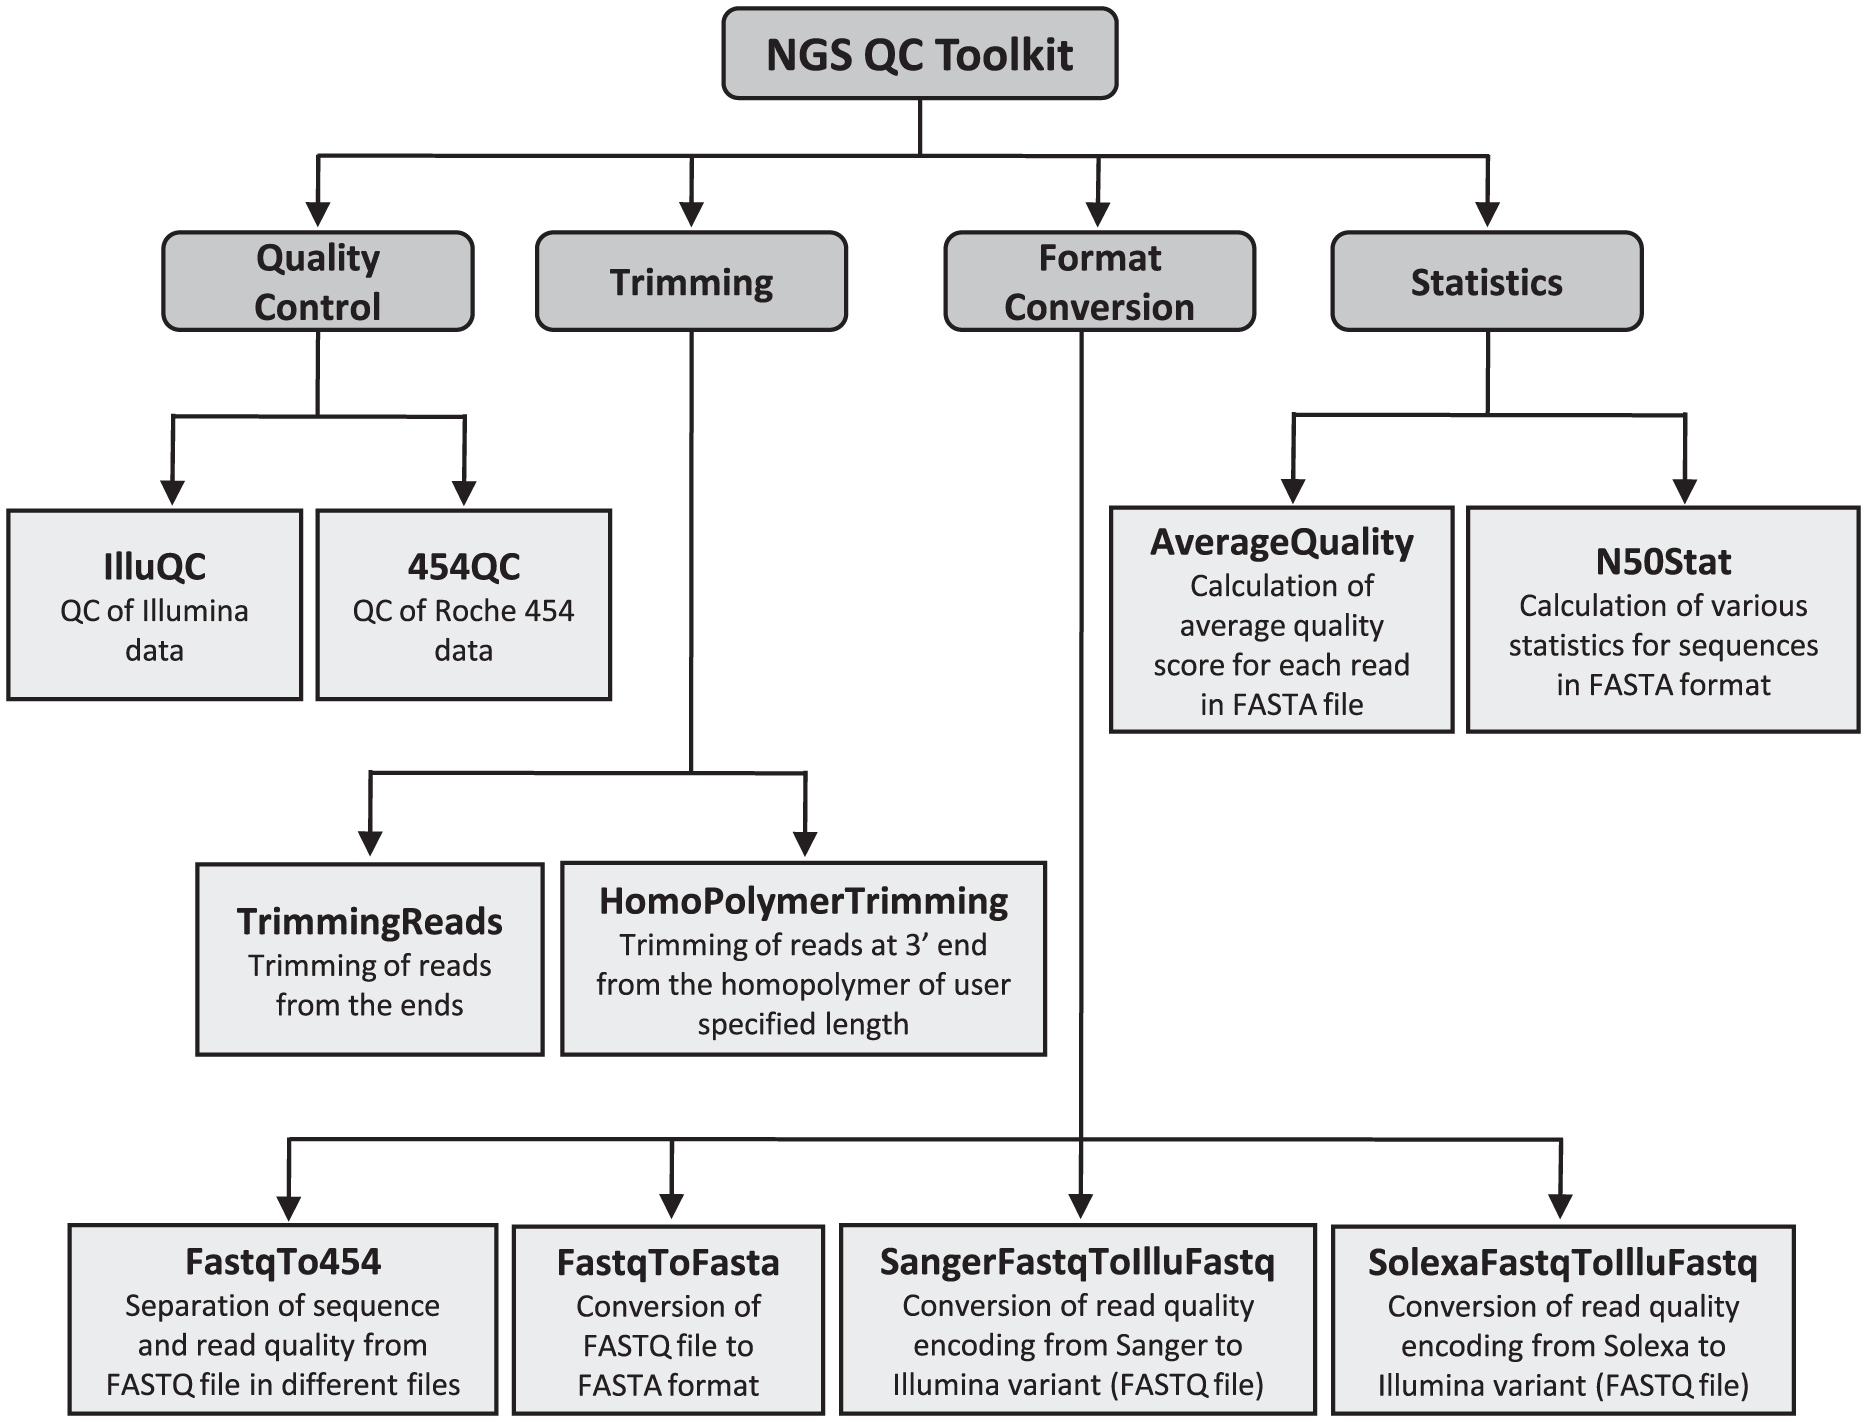
\includegraphics[width=0.9\linewidth]{ngsqc}
	\caption{Flow chart showing various tools included in NGS QC Toolkit.}
	\label{fig:fastqc}
\end{figure}


\section{Ten steps to get started in Genome Assembly and Annotation}
The advice here presented is based on a need seen while working in the ELIXIR-EXCELERATE task “Capacity Building in Genome Assembly and Annotation”. In this capacity we have held courses and workshops in several European countries and have encountered many users in need of a document to support them when they plan and execute their projects. With these 10 steps we aim to fill this need\cite{del2018ten}.

In a de novo genome assembly and annotation project, the nucleotide sequence of a genome is first assembled, as completely as possible, and then annotated. The annotation process infers the structure and function of the assembled sequences. Protein-coding genes are often annotated first, but other features, such as non-coding RNAs or presence of regulatory or repetitive sequences, can also be annotated (Figure~\ref{fig:ngssteps}).

A checklist of things to keep in mind when starting a genome project:

\begin{itemize}
	\item For the DNA extraction, select an individual which is a good representative of the species, and able to provide enough DNA.
	
	\item Extract more DNA than you think you need, or save tissue to use for DNA extraction later. If you need to produce more data later, it is critical to be able to use the same DNA to make sure the data assembles together
	
	\item Remember to extract RNA and order RNA-sequencing if you want to use assembled transcripts in your annotation (which is strongly recommended). If possible, extract RNA from the same individual as used in the DNA extraction to make sure that the RNA-seq reads will map well to your assembly.
	
	\item Decide early on which sequencing technology you will be using, and also consider which assembly tools you want to try. These two choices will greatly influence what kind of compute resources you will need, and you do not want to end in a situation where you have data that you cannot analyze anywhere. Plan compute resources accordingly.
	
\end{itemize}
\begin{figure}
	\centering
	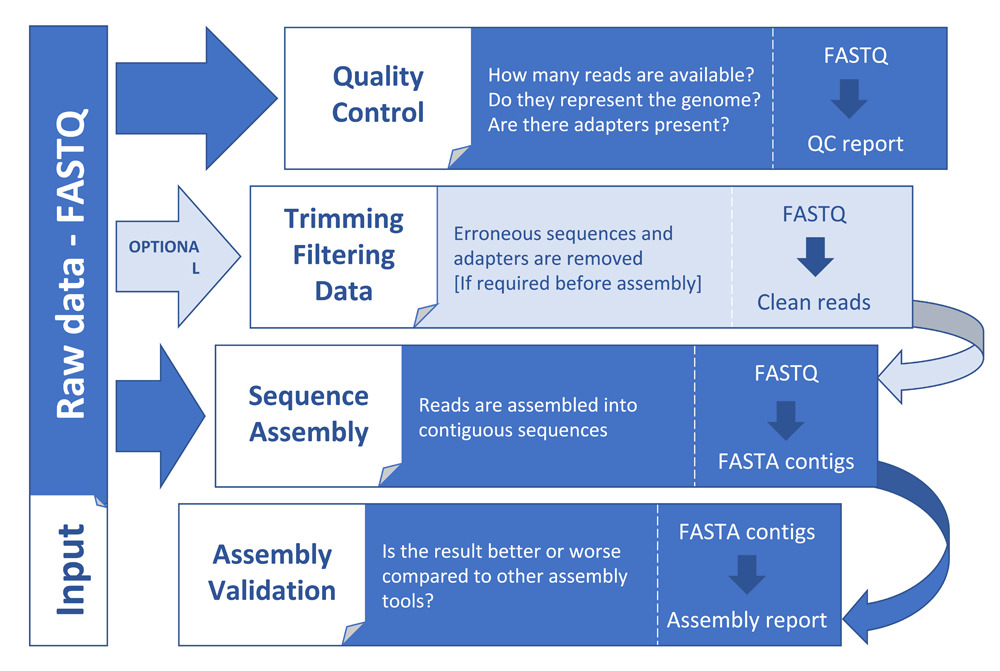
\includegraphics[width=0.9\linewidth]{ngseq}
	\caption{teps to get started in Genome Assembly and Annotation.}
	\label{fig:ngssteps}
\end{figure}

